\documentclass[]{article}

\usepackage{tikz}
\usepackage{amsmath}
\usepackage{amsfonts}
\usepackage{amssymb}
\usepackage{tkz-base}
\usepackage{tkz-euclide}
\usepackage{xcolor}
\usepackage{pgfplots}

% Required package
\usetikzlibrary{positioning}
\usetikzlibrary{svg.path}
\usetikzlibrary{arrows}
\usetikzlibrary{shapes.geometric,calc}

\newdimen\XCoord
\newdimen\YCoord
\newcommand*{\ExtractCoordinate}[1]{\path (#1); \pgfgetlastxy{\XCoord}{\YCoord};}%

%opening
\title{Operational Space Control}
\author{Glen Henshaw\\Craig Carignan}

\begin{document}

\maketitle

\section{Backtracking}
Last time we talked about computed torque control, the most common form of ``true'' nonlinear control used in robotics (as opposed to gain scheduling, which is a form of nonlinear control that treats the robot as if it has linear dynamics, and then uses \textit{ad hoc} techniques to make up for the fact that it doesn't.

Computed torque control is in fact a specific type of a more general control technique called ``alpha--beta partitioning''. The term refers to the fact that when dealing with a nonlinear dynamic system, we often want to have a controller with two parts: a model part that attempts to cancel the natural dynamics, and a feedback part that then instituted new, stable, linear dynamics and in the process takes care of any inaccuracies in the model. This basic idea appears all over nonlinear control and is not restricted to robots.

We can easily see this distinction if we think about controlling a nonlinear spring--mass--damper:
\begin{equation}
 m\ddot{x}+b\dot{x}+qx^{3} = f
\end{equation}
where we have a nonlinear spring in that third term. The control law is going to have the form
\begin{displaymath}
 f = \alpha f' + \beta
\end{displaymath}
where
\begin{eqnarray}
 \alpha & = & m \nonumber \\
 \beta & = & b\dot{x} + qx^{3} \nonumber
\end{eqnarray}
and the servo portion is
\begin{displaymath}
 f = \ddot{x}_{d} + k_{v}\dot{e}+k_{p}e
\end{displaymath}

If we assume we know the dynamics perfectly, and can therefore cancel them exactly, then we're just left with a dynamic system where the error is clearly stable, by inspection:
\begin{eqnarray}
  m\ddot{x}+b\dot{x}+qx^{3} & = & m\left(\ddot{x}_{d} + k_{v}\dot{e}+k_{p}e\right) +b\dot{x}+qx^{3} \nonumber \\
  \Rightarrow 0 & = & \ddot{e} + k_{v}\dot{e} + k_{p}e \nonumber
\end{eqnarray}

If we assume that we don't know the model perfectly, then we need to resort to Lyapunov theory (or some other form of nonlinear analysis). NOTE: there is no ironclad guarantee that such a controller is stable (although it often is -- the presence of a linear feedback servo term makes this framework  \textit{extremely} robust to model uncertainties assuming the gains chosen are ``big enough'' in some informal sense that has to do with both the amount of uncertainty in the model and the bandwidth of the desired trajectory).

Recalling the computed torque control from last week:
\begin{equation}
 \underline{\tau} = M(\underline{\theta})( \ddot{\underline{\theta}}_{d}- K_{p}(\underline{\theta} - \underline{\theta}_{d}) - K_{v}(\underline{\dot{\theta}} - \underline{\dot{\theta}}_{d})) +C(\underline{\theta}, \underline{\dot{\theta}})\dot{\theta} + E(\underline{\theta}, \underline{\dot{\theta}})  \label{computedtorque}
\end{equation}
you can see that in this case
\begin{eqnarray}
 \alpha & = & M(\underline{\theta}) \nonumber \\
 \beta & = & C(\underline{\theta}, \underline{\dot{\theta}})\dot{\theta} + E(\underline{\theta}, \underline{\dot{\theta}}) \nonumber \\
 f' & = & \ddot{\underline{\theta}}_{d}- K_{p}(\underline{\theta} - \underline{\theta}_{d}) - K_{v}(\underline{\dot{\theta}} - \underline{\dot{\theta}}_{d}) \nonumber
\end{eqnarray}

\section{Intro}

Remember from last time that we can write the dynamics of our robot in the form
\begin{equation}
 \underline{\tau} = M(\underline{\theta}) \ddot{\underline{\theta}} +C(\underline{\theta}, \underline{\dot{\theta}})\dot{\theta} + E(\underline{\theta}, \underline{\dot{\theta}}) \label{hamiltonian}
\end{equation}
This is, essentially, a joint--space approach to control. The fundamental problem with joint--space (also known as configuration space) control is that we almost always want to specify the motions of our robotic arm in terms of Cartesian moves of the end effector. We have good inverse kinematics schemes, which let us do this, but by now we're building up a fairly complex set of algorithms, and sometimes it's easier and better to just design our control laws directly in operational space.

\section{Joint--Based Control Architecture}
One approach, of course, is to just specify the trajectory in Cartesian space, use inverse kinematics to convert it to joint space, and then do the control as we've already discussed. Here's a block diagram of our robotic system:

\begin{figure}[h!]
 \centering
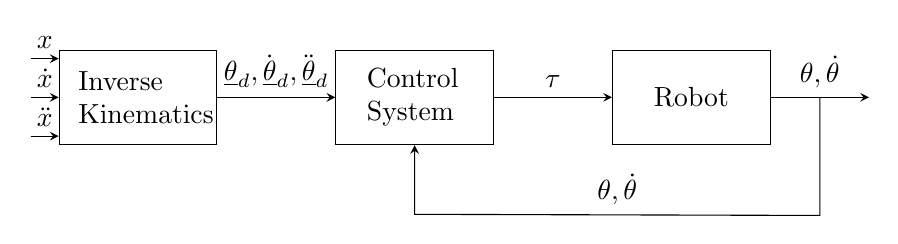
\begin{tikzpicture}
 % Sum shape
 \
 \node[draw, 
        minimum width=2cm,
        minimum height=1.2cm
        ] (trajgen) at (0,0){\parbox[t]{0.125\linewidth}{Inverse\\Kinematics}};

% Controller
\node [draw,
    minimum width=2cm,
    minimum height=1.2cm,
    right=1.5cm of trajgen
]  (controller) {\parbox[t]{0.1\linewidth}{Control\\System}};
 
% System H(s)
\node [draw,
    minimum width=2cm, 
    minimum height=1.2cm,
    right=1.5cm of controller
] (system) {Robot};
  
% Arrows with text label
%\draw[-stealth] (trajgen.north east) -- (controller.north west)
%    node[midway,above]{$\Omega$};
\draw[-stealth] (trajgen.east) -- (controller.west)
    node[midway,above]{$\underline{\theta}_{d}, \dot{\underline{\theta}}_{d}, \ddot{\underline{\theta}}_{d}$};
%\draw[-stealth] (trajgen.south east) -- (controller.south west)
%    node[midway,above]{$\ddot{\Omega}$};
 
\draw[-stealth] (controller.east) -- (system.west) 
    node[midway,above]{$\tau$};

\draw[-stealth] (system.east) -- ++ (1.25,0) 
    node[midway](output){}node[midway,above]{$\theta, \dot{\theta}$};

\ExtractCoordinate{controller.south}
\draw[-stealth] (output.center) -- ++ (0,-1.5) -- (\XCoord, \YCoord-25) node[midway,above]{$\theta, \dot{\theta}$} -- (controller.south);

\ExtractCoordinate{trajgen.west}
\draw[-stealth] (\XCoord-10, \YCoord+14) -- (\XCoord, \YCoord+14) node[midway,above]{$x$};
\draw[-stealth] (\XCoord-10, \YCoord) -- (\XCoord, \YCoord) node[midway,above]{$\dot{x}$};
\draw[-stealth] (\XCoord-10, \YCoord-14) -- (\XCoord, \YCoord-14) node[midway,above]{$\ddot{x}$};
  
\end{tikzpicture}
\end{figure}

where the inverse kinematics equations look like:
\begin{eqnarray}
\underline{q}_{d} & = & f^{-1}(\underline{x}_{d}) \nonumber \\
\underline{\dot{q}}_{d} & = & J^{-1}(\underline{q}_{d})\underline{\dot{x}}_{d} \nonumber \\
\underline{\ddot{q}}_{d} & = & \dot{J}^{-1}\underline{\dot{x}}_{d} + J^{-1}\underline{\ddot{x}}_{d} \nonumber
\end{eqnarray}
...and finding that second derivative might be tricky. In practice, it's often done using a numerical difference scheme, which works in most cases because we're differencing something that has no noise. But it isn't ideal.

\section{Operational Space Control}
\subsection{Inverse Jacobian Control}
Here's one way to approach Cartesian space control:

\begin{figure}[h!]
 \centering
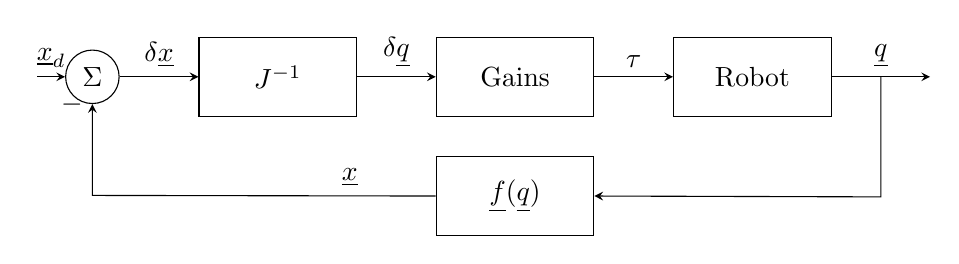
\begin{tikzpicture}
 % Sum shape
 \node[circle,draw, minimum width=0.5cm] (sum) at (-1,0){$\Sigma$} ;
 \node[draw, 
        minimum width=2cm,
        minimum height=1cm,
        right=1cm of sum
        ] (trajgen) {$J^{-1}$};

% Controller
\node [draw,
    minimum width=2cm,
    minimum height=1cm,
    right=1cm of trajgen
]  (controller) {Gains};
 
% System H(s)
\node [draw,
    minimum width=2cm, 
    minimum height=1cm,
    right=1cm of controller
] (system) {Robot};

\node [draw,
    minimum width=2cm, 
    minimum height=1cm,
    below=0.5cm of controller
] (fkine) {$\underline{f}(\underline{q})$};
% Arrows with text label
%\draw[-stealth] (trajgen.north east) -- (controller.north west)
%    node[midway,above]{$\Omega$};
\draw[-stealth] (trajgen.east) -- (controller.west)
    node[midway,above]{$\delta \underline{q}$};
%\draw[-stealth] (trajgen.south east) -- (controller.south west)
%    node[midway,above]{$\ddot{\Omega}$};

\draw[-stealth] (sum.east) -- (trajgen.west) node[midway,above](x){$\delta\underline{x}$};
\draw[-stealth] (controller.east) -- (system.west) 
    node[midway,above]{$\tau$};

\draw[-stealth] (system.east) -- ++ (1.25,0) 
    node[midway](output){}node[midway,above]{$\underline{q}$};

\draw[-stealth] (output.center) -- ++ (0,-1.525) -- (fkine.east);

\ExtractCoordinate{sum.west}
\draw[-stealth] (\XCoord-10, \YCoord) -- (\XCoord, \YCoord) node[midway,above]{$\underline{x}_{d}$};
\ExtractCoordinate{sum.south}
\draw[-stealth] (fkine.west) -- (\XCoord, \YCoord-33) node[pos=0.25,above]{$\underline{x}$} -- (sum.south) node[below,left]{$-$};

\end{tikzpicture}
\end{figure}

Note that $\underline{x}_{d}-\underline{x} \approx J(\underline{q}_{d}-\underline{q})$ for small errors.

This has two problems:
\begin{enumerate}
 \item It's unstable near singularities
 \item That inverse calculation can be computationally complex. This used to be a bigger problem, when embedded computers were a lot slower at floating point computations, but it still can crop up, e.g. if you're trying to operate a rover on the surface of Venus or something similarly insane.
\end{enumerate}
\pagebreak
\subsection{Jacobian Transpose Control}
If you \textit{are} trying to build a rover for the surface of Venus, and you just can't deal with modern CPUs, there's a fascinating approach that doesn't require taking an inverse. It's also very, very stable.

\begin{figure}[h!]
 \centering
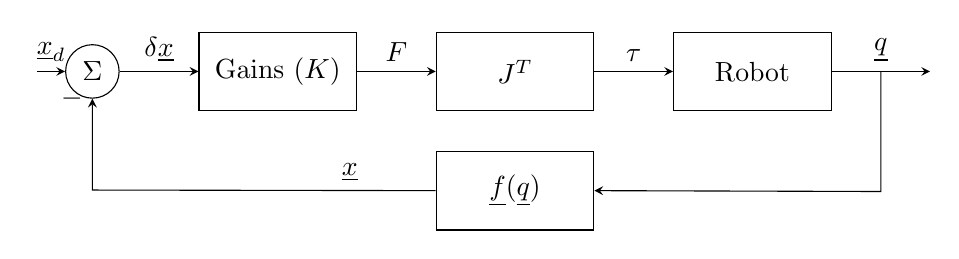
\begin{tikzpicture}
 % Sum shape
 \node[circle,draw, minimum width=0.5cm] (sum) at (-1,0){$\Sigma$} ;
 \node[draw, 
        minimum width=2cm,
        minimum height=1cm,
        right=1cm of sum
        ] (trajgen) {Gains ($K$)};

% Controller
\node [draw,
    minimum width=2cm,
    minimum height=1cm,
    right=1cm of trajgen
]  (controller) {$J^{T}$};
 
% System H(s)
\node [draw,
    minimum width=2cm, 
    minimum height=1cm,
    right=1cm of controller
] (system) {Robot};

\node [draw,
    minimum width=2cm, 
    minimum height=1cm,
    below=0.5cm of controller
] (fkine) {$\underline{f}(\underline{q})$};
% Arrows with text label
%\draw[-stealth] (trajgen.north east) -- (controller.north west)
%    node[midway,above]{$\Omega$};
\draw[-stealth] (trajgen.east) -- (controller.west)
    node[midway,above]{$F$};
%\draw[-stealth] (trajgen.south east) -- (controller.south west)
%    node[midway,above]{$\ddot{\Omega}$};

\draw[-stealth] (sum.east) -- (trajgen.west) node[midway,above](x){$\delta\underline{x}$};
\draw[-stealth] (controller.east) -- (system.west) 
    node[midway,above]{$\tau$};

\draw[-stealth] (system.east) -- ++ (1.25,0) 
    node[midway](output){}node[midway,above]{$\underline{q}$};

\draw[-stealth] (output.center) -- ++ (0,-1.525) -- (fkine.east);

\ExtractCoordinate{sum.west}
\draw[-stealth] (\XCoord-10, \YCoord) -- (\XCoord, \YCoord) node[midway,above]{$\underline{x}_{d}$};
\ExtractCoordinate{sum.south}
\draw[-stealth] (fkine.west) -- (\XCoord, \YCoord-33) node[pos=0.25,above]{$\underline{x}$} -- (sum.south) node[below,left]{$-$};

\end{tikzpicture}
\end{figure}
...where the idea is that we use the fact that the Jacobian transpose converts Cartesian forces to joint torques:
\begin{displaymath}
 \underline{\tau} = J^{T}\underline{F}
\end{displaymath}
so what we're doing here is using our gains to calculate a fictional Cartesian force, and then converting that force to joint torques, thus approximating those forces.

This also has some issues:
\begin{enumerate}
 \item $\underline{\tau} = J^{T}\underline{F}$ ignores dynamics. It ``behaves'' as if the arm is an ideal kinematic system; and
 \item $\underline{F}=K\ \delta\underline{x}$ is a static relationship.
\end{enumerate}

\subsubsection{Example}
Here's an example, doing it both ways.

Our old friend the two--link planar manipulator:
\begin{figure}[!h]
\centering
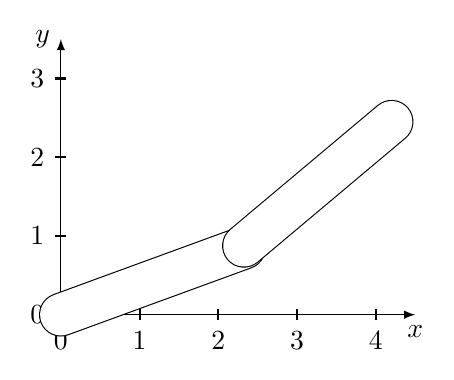
\begin{tikzpicture}
\tkzInit[xmax=4,ymax=3,xmin=0,ymin=0]
%\tkzGrid
\tkzAxeXY
\draw[cm={0.93,0.34,-0.34,0.93,(0,0)}][double=none, double distance=15pt, line join=round, line cap=round] (0.0, 0.0) -- (2.5, 0);
%\draw[cm={0.93,0.34,-0.34,0.93,(0, 0)}][->][line width=1mm] (0.5, -0.35) arc (-25:25:1cm) node[ label=above:$\tau$]{ };
\draw[cm={0.75,0.63,-0.63,0.75,(2.325, 0.875)}][double=none, double distance=15pt, line join=round, line cap=round] (0.0, 0.0) -- (2.5, 0);
%\draw[cm={0.75,0.63,-0.63,0.75,(2.325, 0.875)}][->][line width=1mm] (0.5, -0.35) arc (-25:25:1cm) node[ label=above:$\tau$]{ };
%\draw[->][cm={1.0, 0.0, 0.0, 1.0,(4.19, 2.5)}][line width=1mm] (2.0, 0.0) -- (0.0, 0.0) node[ label=above:$\underline{f}$]{ };;
\end{tikzpicture}
\end{figure}

where

\begin{displaymath}
 J = \left[\begin{array}{cc} -l_{1}s_{1}-l_{2}s_{12} & -l_{2}s_{12} \\ l_{1}c_{1}+l_{2}c_{12} & l_{2}c_{12} \end{array} \right]
\end{displaymath}

Let's examine it at $\theta_{1} = \theta_{2} = 0$:
\begin{displaymath}
 J = \left[\begin{array}{cc} 0 & 0 \\ l_{1}+l_{2} & l_{2} \end{array} \right]
\end{displaymath}
\begin{enumerate}
 \item $J^{-1}$ control:
 \begin{displaymath}
  \underline{\dot{x}} = J\underline{\dot{\theta}}
 \end{displaymath}
so
\begin{eqnarray}
 \dot{x} & = & 0 \nonumber \\
 \dot{y} & = & (l_{1}+l_{2})\dot{\theta_{1}} + l_{2}\dot{\theta_{2}} \nonumber
\end{eqnarray}
which indicates that motion in the $x$ direction is not possible. Which makes sense, this is a singular pose. When we try to do the Jacobian inversion, then, $J^{-1}$ explodes.
\item $J^{T}$ Control
\begin{eqnarray}=
 \underline{\tau} & = & J^{T}\underline{F} \nonumber \\
 \underline{F} & = & K\ \delta\underline{x} \nonumber
\end{eqnarray}
where
\begin{eqnarray}
 \tau_{1} & = & (l_{1}+l_{2})f_{y} \nonumber \\
 \tau_{2} & = & l_{2}f_{y} \nonumber
\end{eqnarray}
...so in this case, commands to move in the $x-$ direction are simply ignored. Which is good, because the arm is physically incapable of moving in the $x-$direction. And you get singularities management, basically for free.
\end{enumerate}

\section{Cartesian Computed Torque Control}
It turns out that it's possible to write the full nonlinear dynamics of a robot in Cartesian terms:
\begin{displaymath}
 H_{x}(\underline{\theta})\ddot{\underline{x}} + C_{x}(\underline{\theta}, \dot{\underline{\theta}}) + E_{x}(\underline{\theta}, \underline{\dot{\theta}}) = \underline{F}
\end{displaymath}
which you can convince yourself enough with the right insertion of Jacobians and derivatives of Jacobians in the right places:
\begin{eqnarray}
	H_{x}(\underline{\theta}) & = & J^{-T}(\underline{\theta})M(\underline{\theta})J^{-1}(\underline{\theta}) \nonumber \\
	C_{x}(\underline{\theta}, \dot{\underline{\theta}}) & = & J^{-T}(\underline{\theta})\left(C(\underline{\theta}, \dot{\underline{\theta}}) - H(\underline{\theta})J^{-1}(\underline{\theta})\dot{J}(\underline{\theta})\dot{\underline{\theta}}\right) \nonumber \\
	E_{x}(\underline{\theta}, \dot{\underline{\theta}}) & = & J^{-T}(\underline{\theta})E(\underline{\theta}, \underline{\dot{\theta}}) \nonumber
\end{eqnarray}
where $J^{-T}$ refers to the transpose of the Jacobian inverse. 

You can then contemplate doing what looks like a Cartesian computed torque controller using the same $\alpha-\beta$ partitioning scheme as before:
\begin{eqnarray}
 \underline{F} & = & H_{x}(\underline{\theta})\underline{F}' + \beta \nonumber \\
 \beta & = & C_{x}(\underline{\theta}, \dot{\underline{\theta}}) + E_{x}(\underline{\theta}, \underline{\dot{\theta}}) \nonumber \\
 \underline{f}' & = & \underline{\ddot{x}}_{d} + K_{p_{x}}(\underline{x}_{d}-\underline{x}) + K_{v_{x}}(\underline{\dot{x}}_{d} - \underline{\dot{x}}) \nonumber
\end{eqnarray}
Note that finding the derivative of the Jacobian is a fairly onerous calculation, which goes a long way towards explaining why these schemes are not more widely used. There are now programming languages that support automatic differentiation, though, so maybe we'll see them become more popular in the future.
\end{document}
